\documentclass[a4paper,12pt]{article}

\usepackage[T2A]{fontenc}
\usepackage[english,russian]{babel}
\usepackage[breakable]{tcolorbox}
\usepackage[utf8]{inputenc}

\usepackage{cmap}
\usepackage{geometry}
\usepackage{hyperref}
\usepackage{setspace}
\usepackage{graphicx}
\usepackage{booktabs}
\usepackage{array}
\usepackage{paralist}
\usepackage{verbatim}
\usepackage{amsmath}
\usepackage{amsfonts}
\usepackage{amssymb}
\usepackage{enumerate}
\usepackage{pifont}
\usepackage{subfig}
\usepackage{indentfirst}
\usepackage{tocbibind}
\usepackage{grffile}
\usepackage{parskip}
\usepackage{caption}
\usepackage{float}
\usepackage{xcolor}
\usepackage{textcomp}
\usepackage{calc}
\usepackage{epstopdf}

\title{
\Huge Оценка эффекта высшего образования на здоровье\par
\vspace{1em}
\large Оценивание влияния высшего образования на здоровье: сравнение многомерной рекурсивной пробит-модели и мэтчинга\par
\large Е.~Коссова, М.~Косорукова
}

\author{\large ФЭН НИУ ВШЭ \\
\large Исследовательский поток, БЭК232 \\
\large Эконометрика-2 (углубленный курс) \\
\\
\large А. Карасев: DoubleML и Оформление текста в \LaTeX \\ 
\large Л. Панчеха: Исследование данных и Мэтчинг \\ 
\large М. Удовиченко: Подготовка данных и Пробит}

\date{\today{}}

\begin{document}

\maketitle{}

\newpage{}

\section{Вступление}

В качестве основы работы взята статья Е. Коссовой и М. Косоруковой \href{https://ideas.repec.org/a/ris/apltrx/0465.html}{"Оценивание влияния высшего образования на здоровье: сравнение многомерной рекурсивной пробит-модели и мэтчинга"}. 
В статье рассматривается эффект высшего образования на здоровье людей. 
Кроме того, ключевой темой статьи является сравнение двух методов оценки эффектов: параметрической многомерной пробит модели с непараметрическим мэтчингом на Propensity Score Matching и расстоянии Махалонобиса. 
Оценки в изучаемой статье вычисляются на основе данных \href{https://www.hse.ru/rlms/}{Российского мониторинга экономического положения и здоровья населения} от НИУ ВШЭ на данных 2019-го года. 

Цель нашего исследования состоит в том, чтобы проверить выводы, сделанные в статьи на данных 2019-года, на данных 2024-го года (полная выборка), чтобы проверить валидность и "долговечность" выводов, сделанных авторами в статье. 

Будем придерживаться следующего плана выполнения проекта:
\begin{itemize}
    \item Знакомство с оригинальной статьёй
    \item Выгрузка и подготовка данных (выбор необходимых полей, их переименование и сопоставление с оригинальной статьёй)
    \item Исследование данных: построение разнообразных графиков, понимание общей структуры исследуемого датасета
    \item Измерение причинно-следственной связи через многомерную рекурсивной пробит модель
    \item Измерение причинно-следственной связи через мэтчинг
    \item Измерение причинно-следственной связи через DoubleML подход
    \item Общие выводы
\end{itemize}

\newpage{}

\section{Исходная статья}

Оригинальная статья имеет две основных повествовательных линии:
\begin{itemize}
    \item Оценка эффекта высшего образования на здоровье индивидов
    \item Сравнение многомерной рекурсивной пробит модели и мэтчинга
\end{itemize}

В оригинальной статье были сделаны следующие выводы:
\begin{enumerate}
    \item Необходимость использование нескольких методов для оценки эффекта 
    (в том числе одновременно параметрических и непараметрическим подходов)
    \item Статистически значимый отрицательный эффект высшего образования на вероятность женщин иметь гипертонию
    \item Статистически значимый отрицательный эффект высшего образования на вероятность женщин иметь избыточный вес (ожирение)
    \item Статистически значимый отрицательный эффект высшего образования на вероятность мужчин оценивать свое здоровье как очень хорошее
    \item Статистически значимый положительный эффект высшего образования на вероятность женщин иметь заболевания глаз
    \item Статистически значимый положительный эффект высшего образования на вероятность женщин иметь аллергию
\end{enumerate}

Мы будем проверять гипотезы 1-2 и 4-6 (данные об избыточном весе отсутствуют в выборке 2024-го года)

\newpage{}

\section{Исследование данных}

Прежде чем приступить к оценки эффекта, проведем краткий разведывательный анализ данных:

\begin{center}
    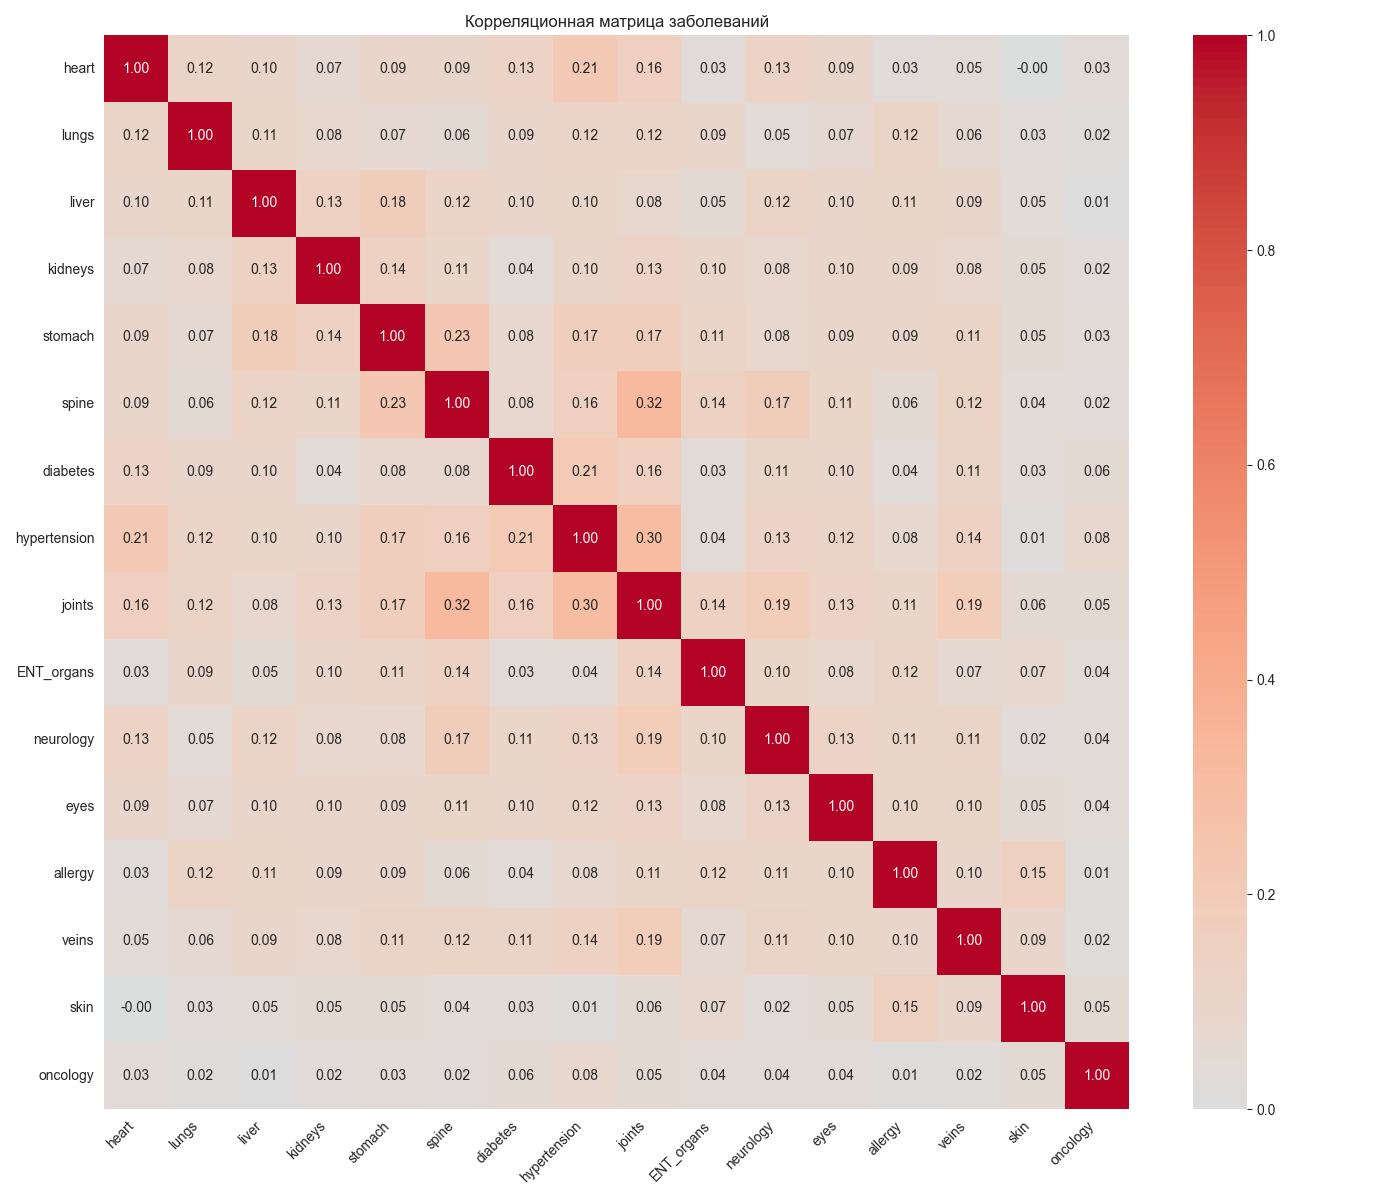
\includegraphics[width=0.8\textwidth]{assets/cor_map.png}
\end{center}

\begin{center}
    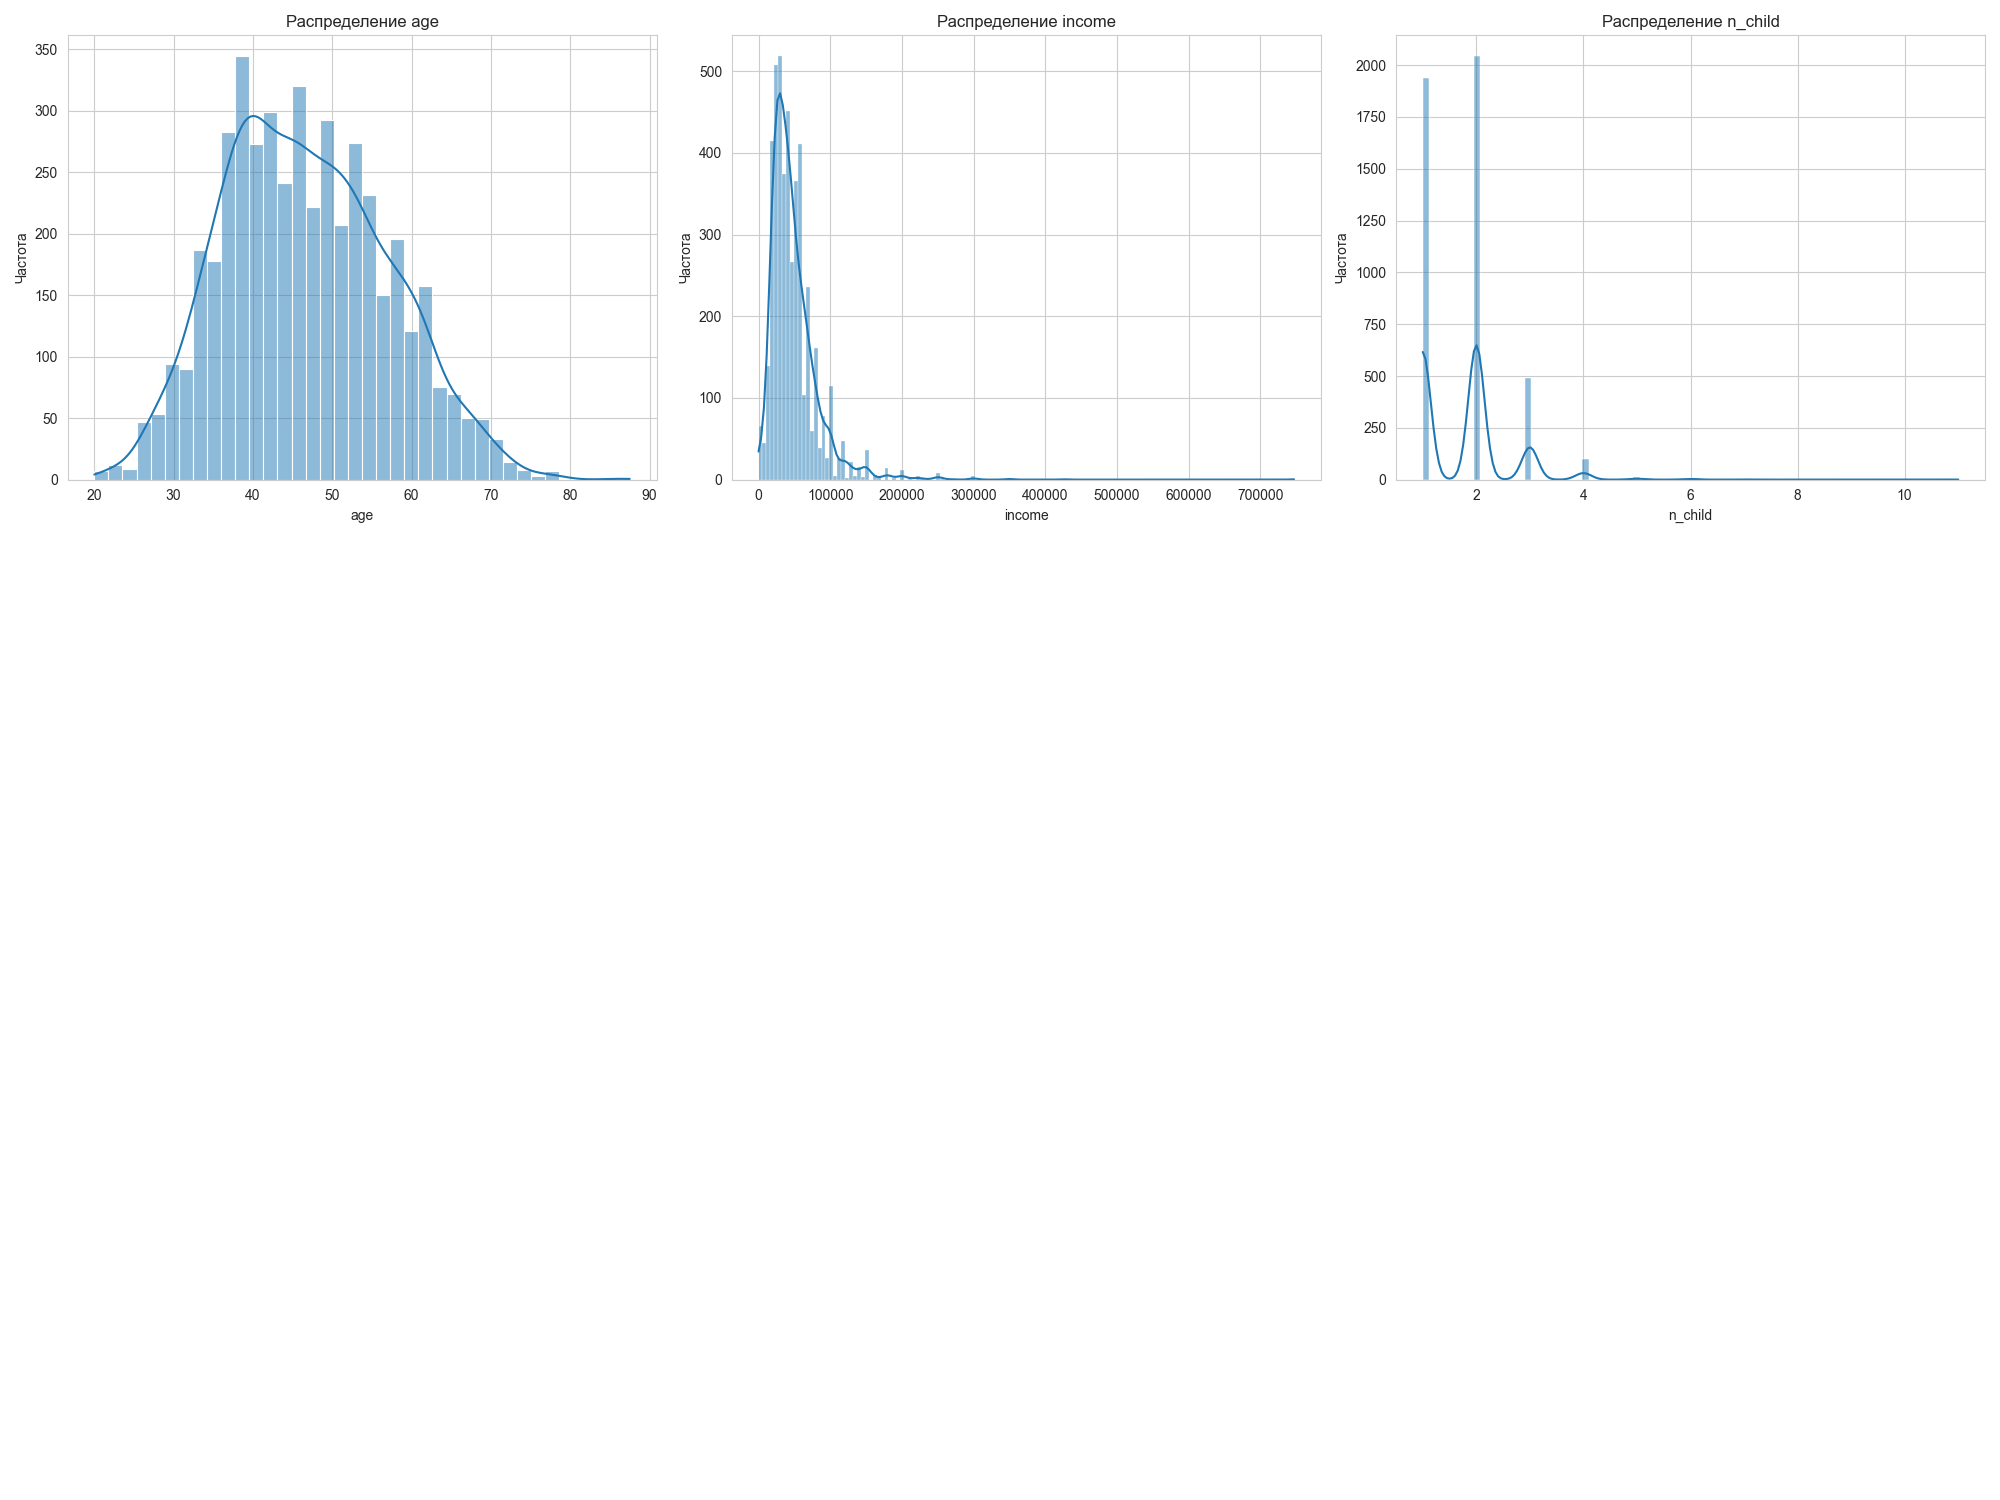
\includegraphics[width=0.8\textwidth]{assets/eda_hist_cont.png}
\end{center}

\begin{center}
    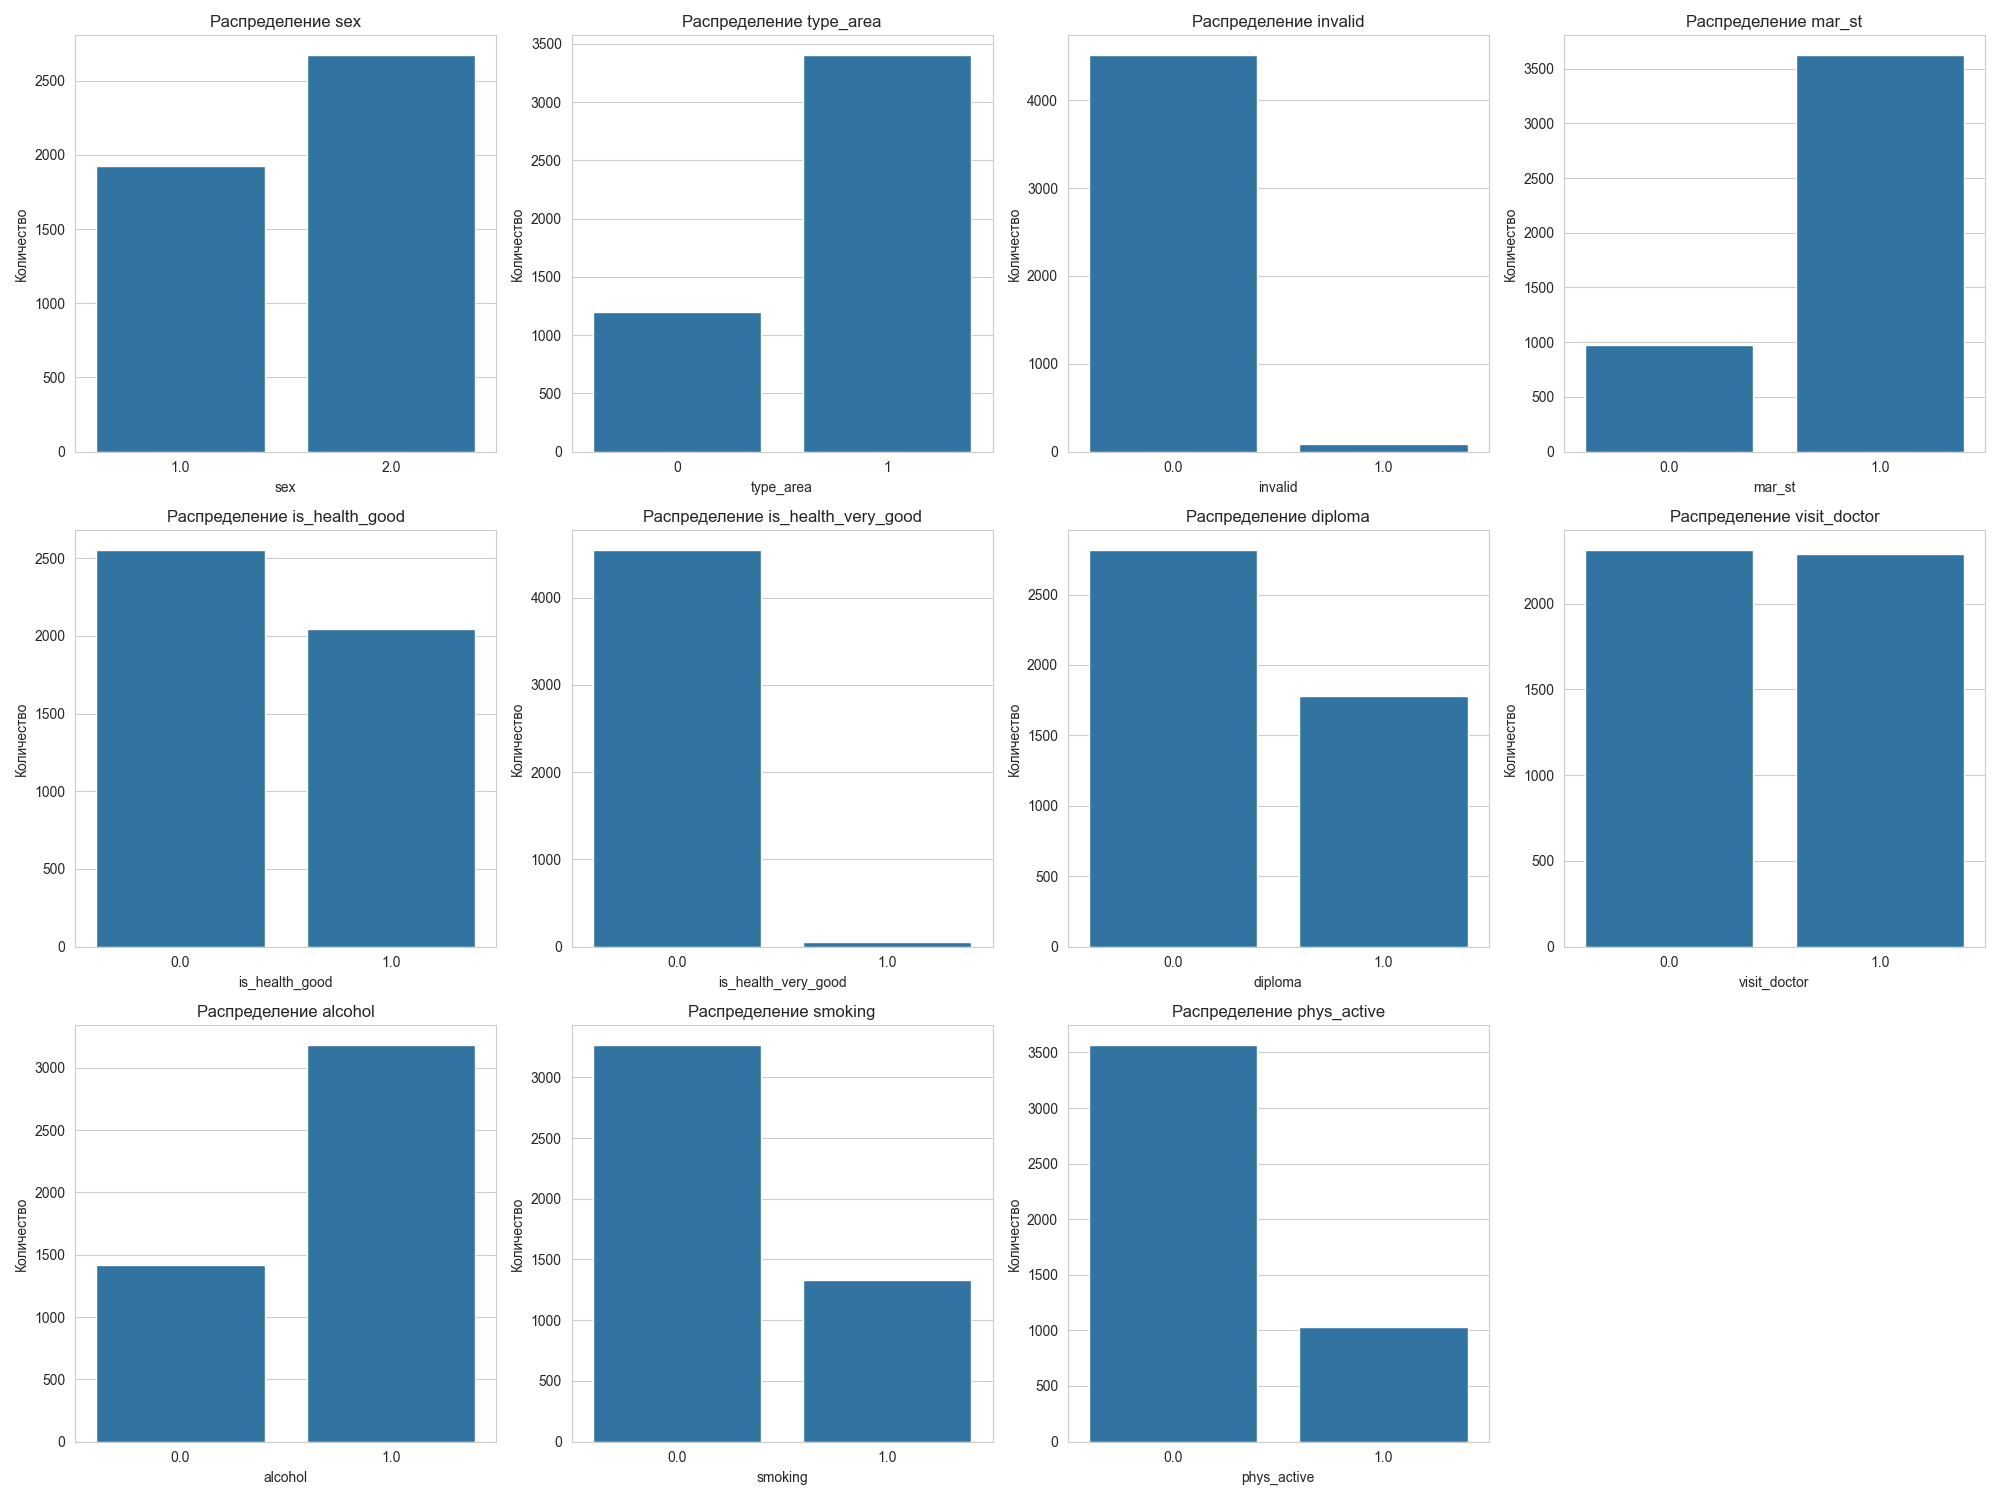
\includegraphics[width=0.8\textwidth]{assets/eda_hist_bin.png}
\end{center}

\begin{center}
    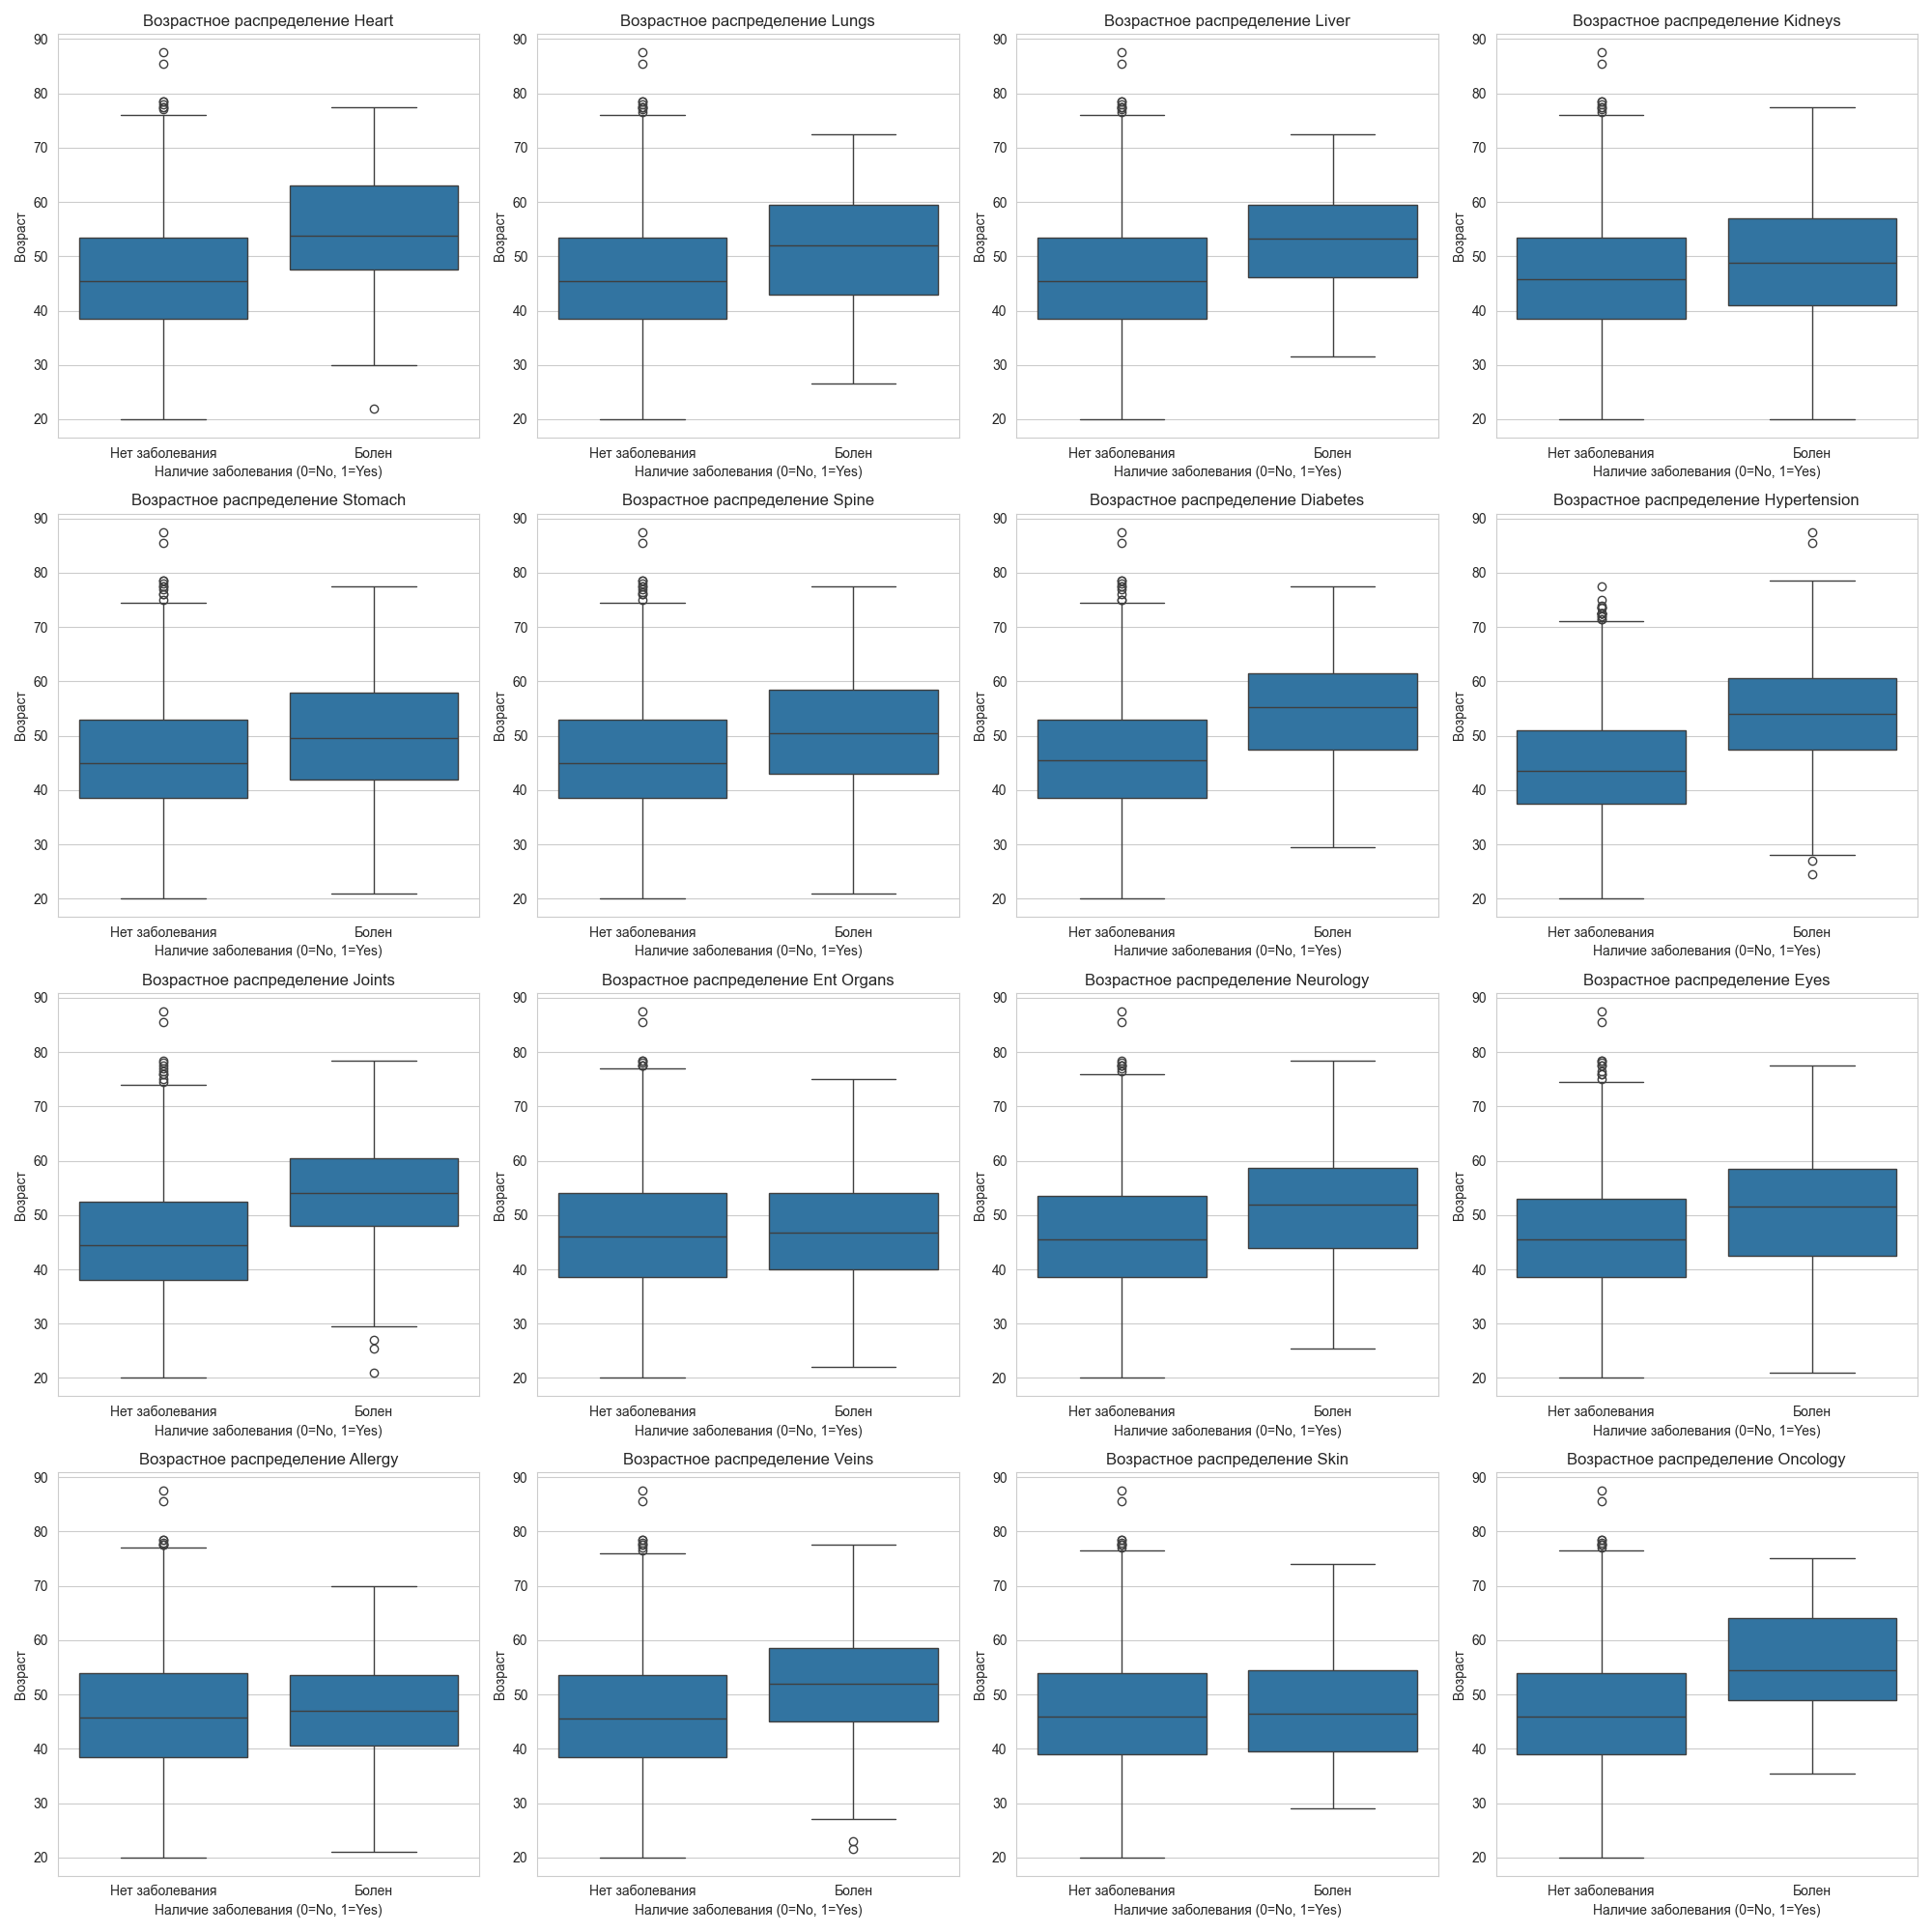
\includegraphics[width=0.8\textwidth]{assets/disease_age_distr.png}
\end{center}

\begin{center}
    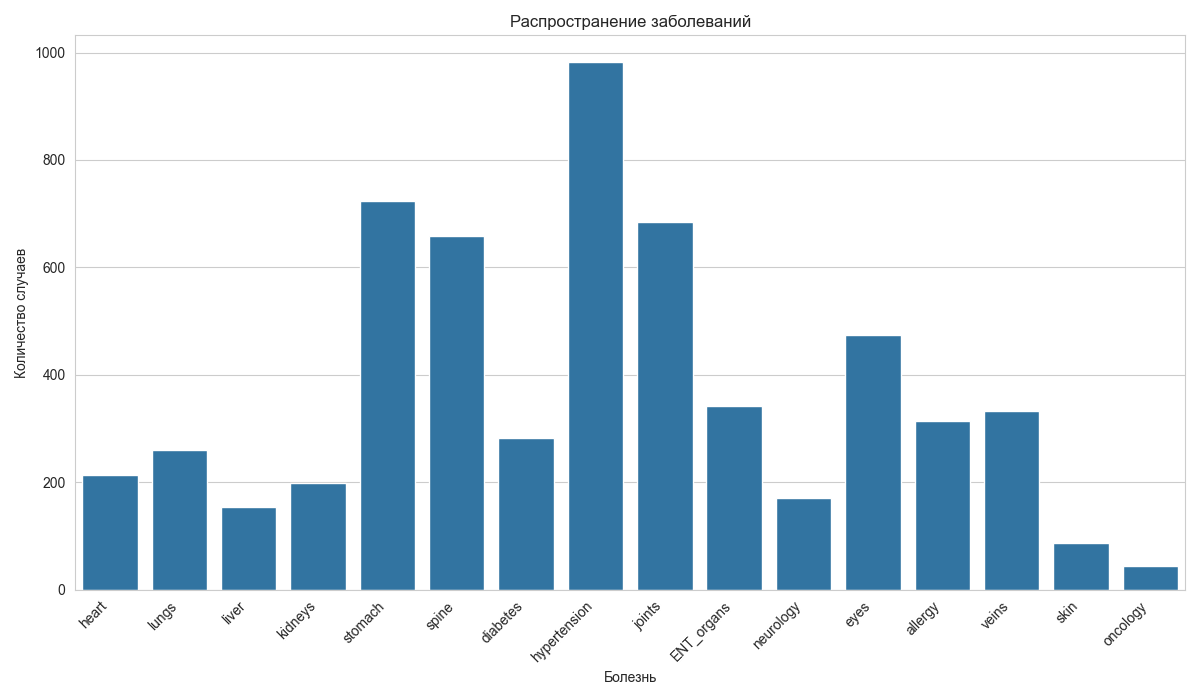
\includegraphics[width=0.8\textwidth]{assets/disease_count.png}
\end{center}

\begin{center}
    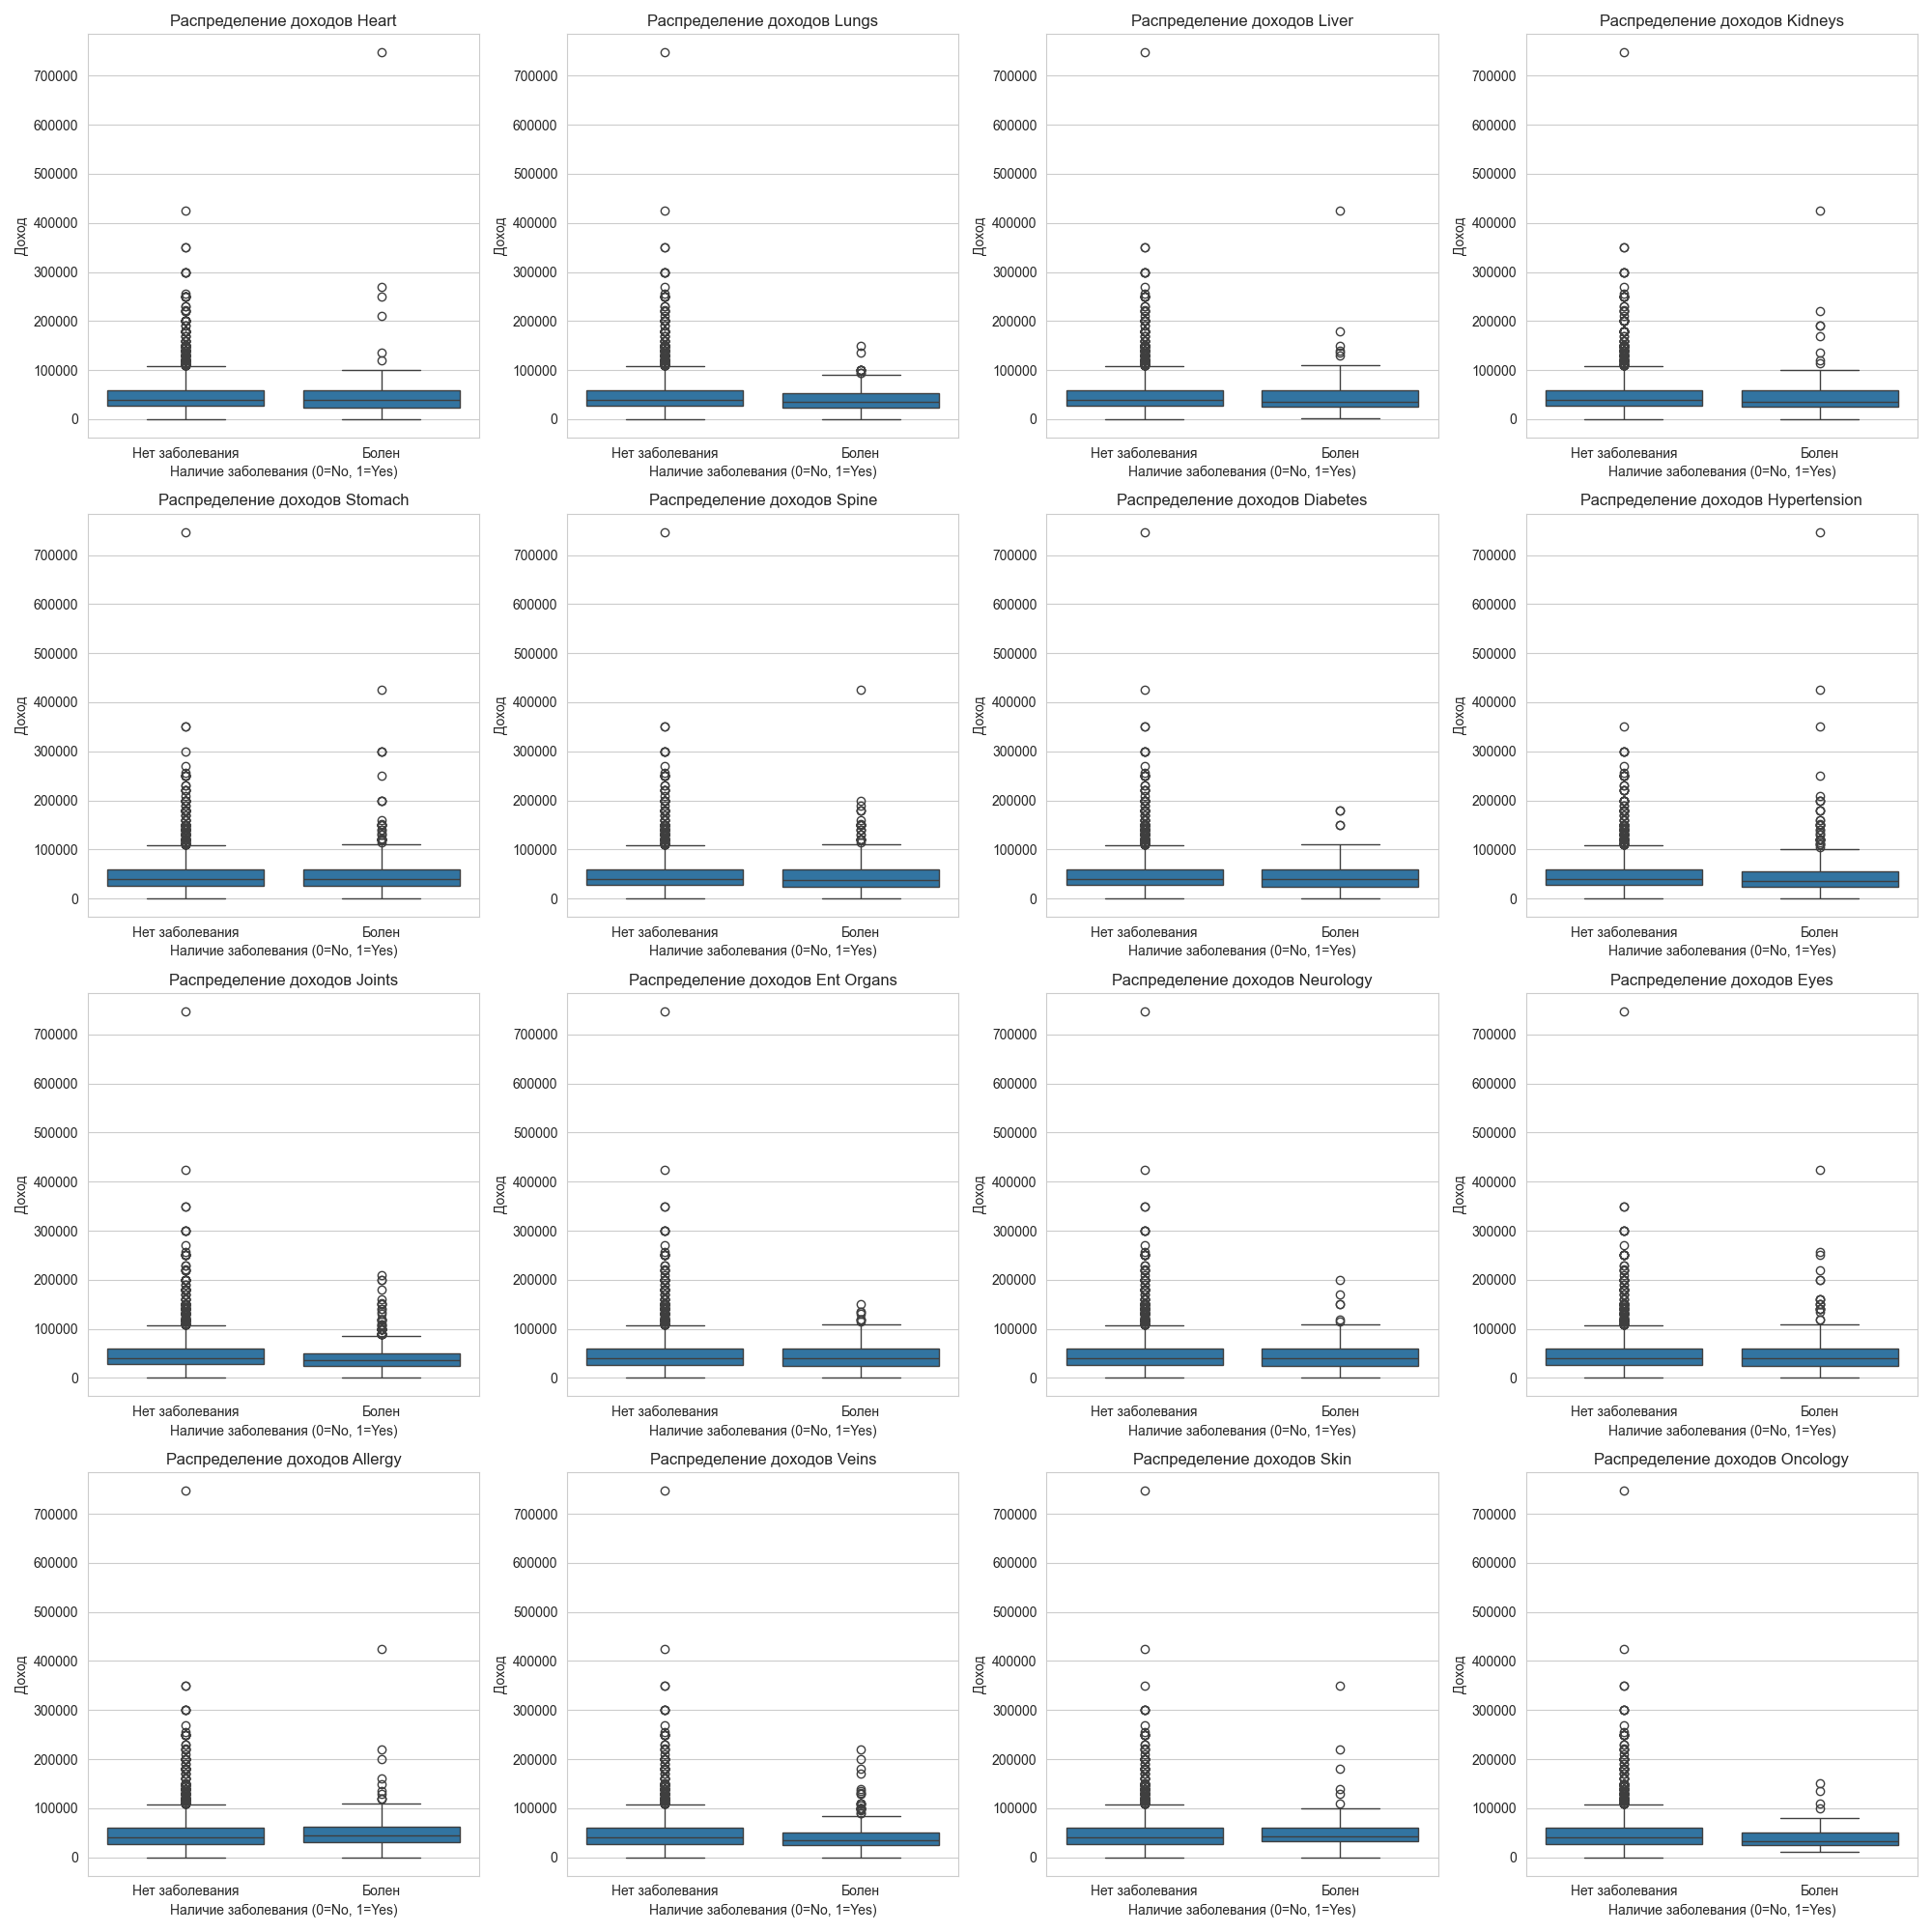
\includegraphics[width=0.8\textwidth]{assets/disease_income_distr.png}
\end{center}

\begin{center}
    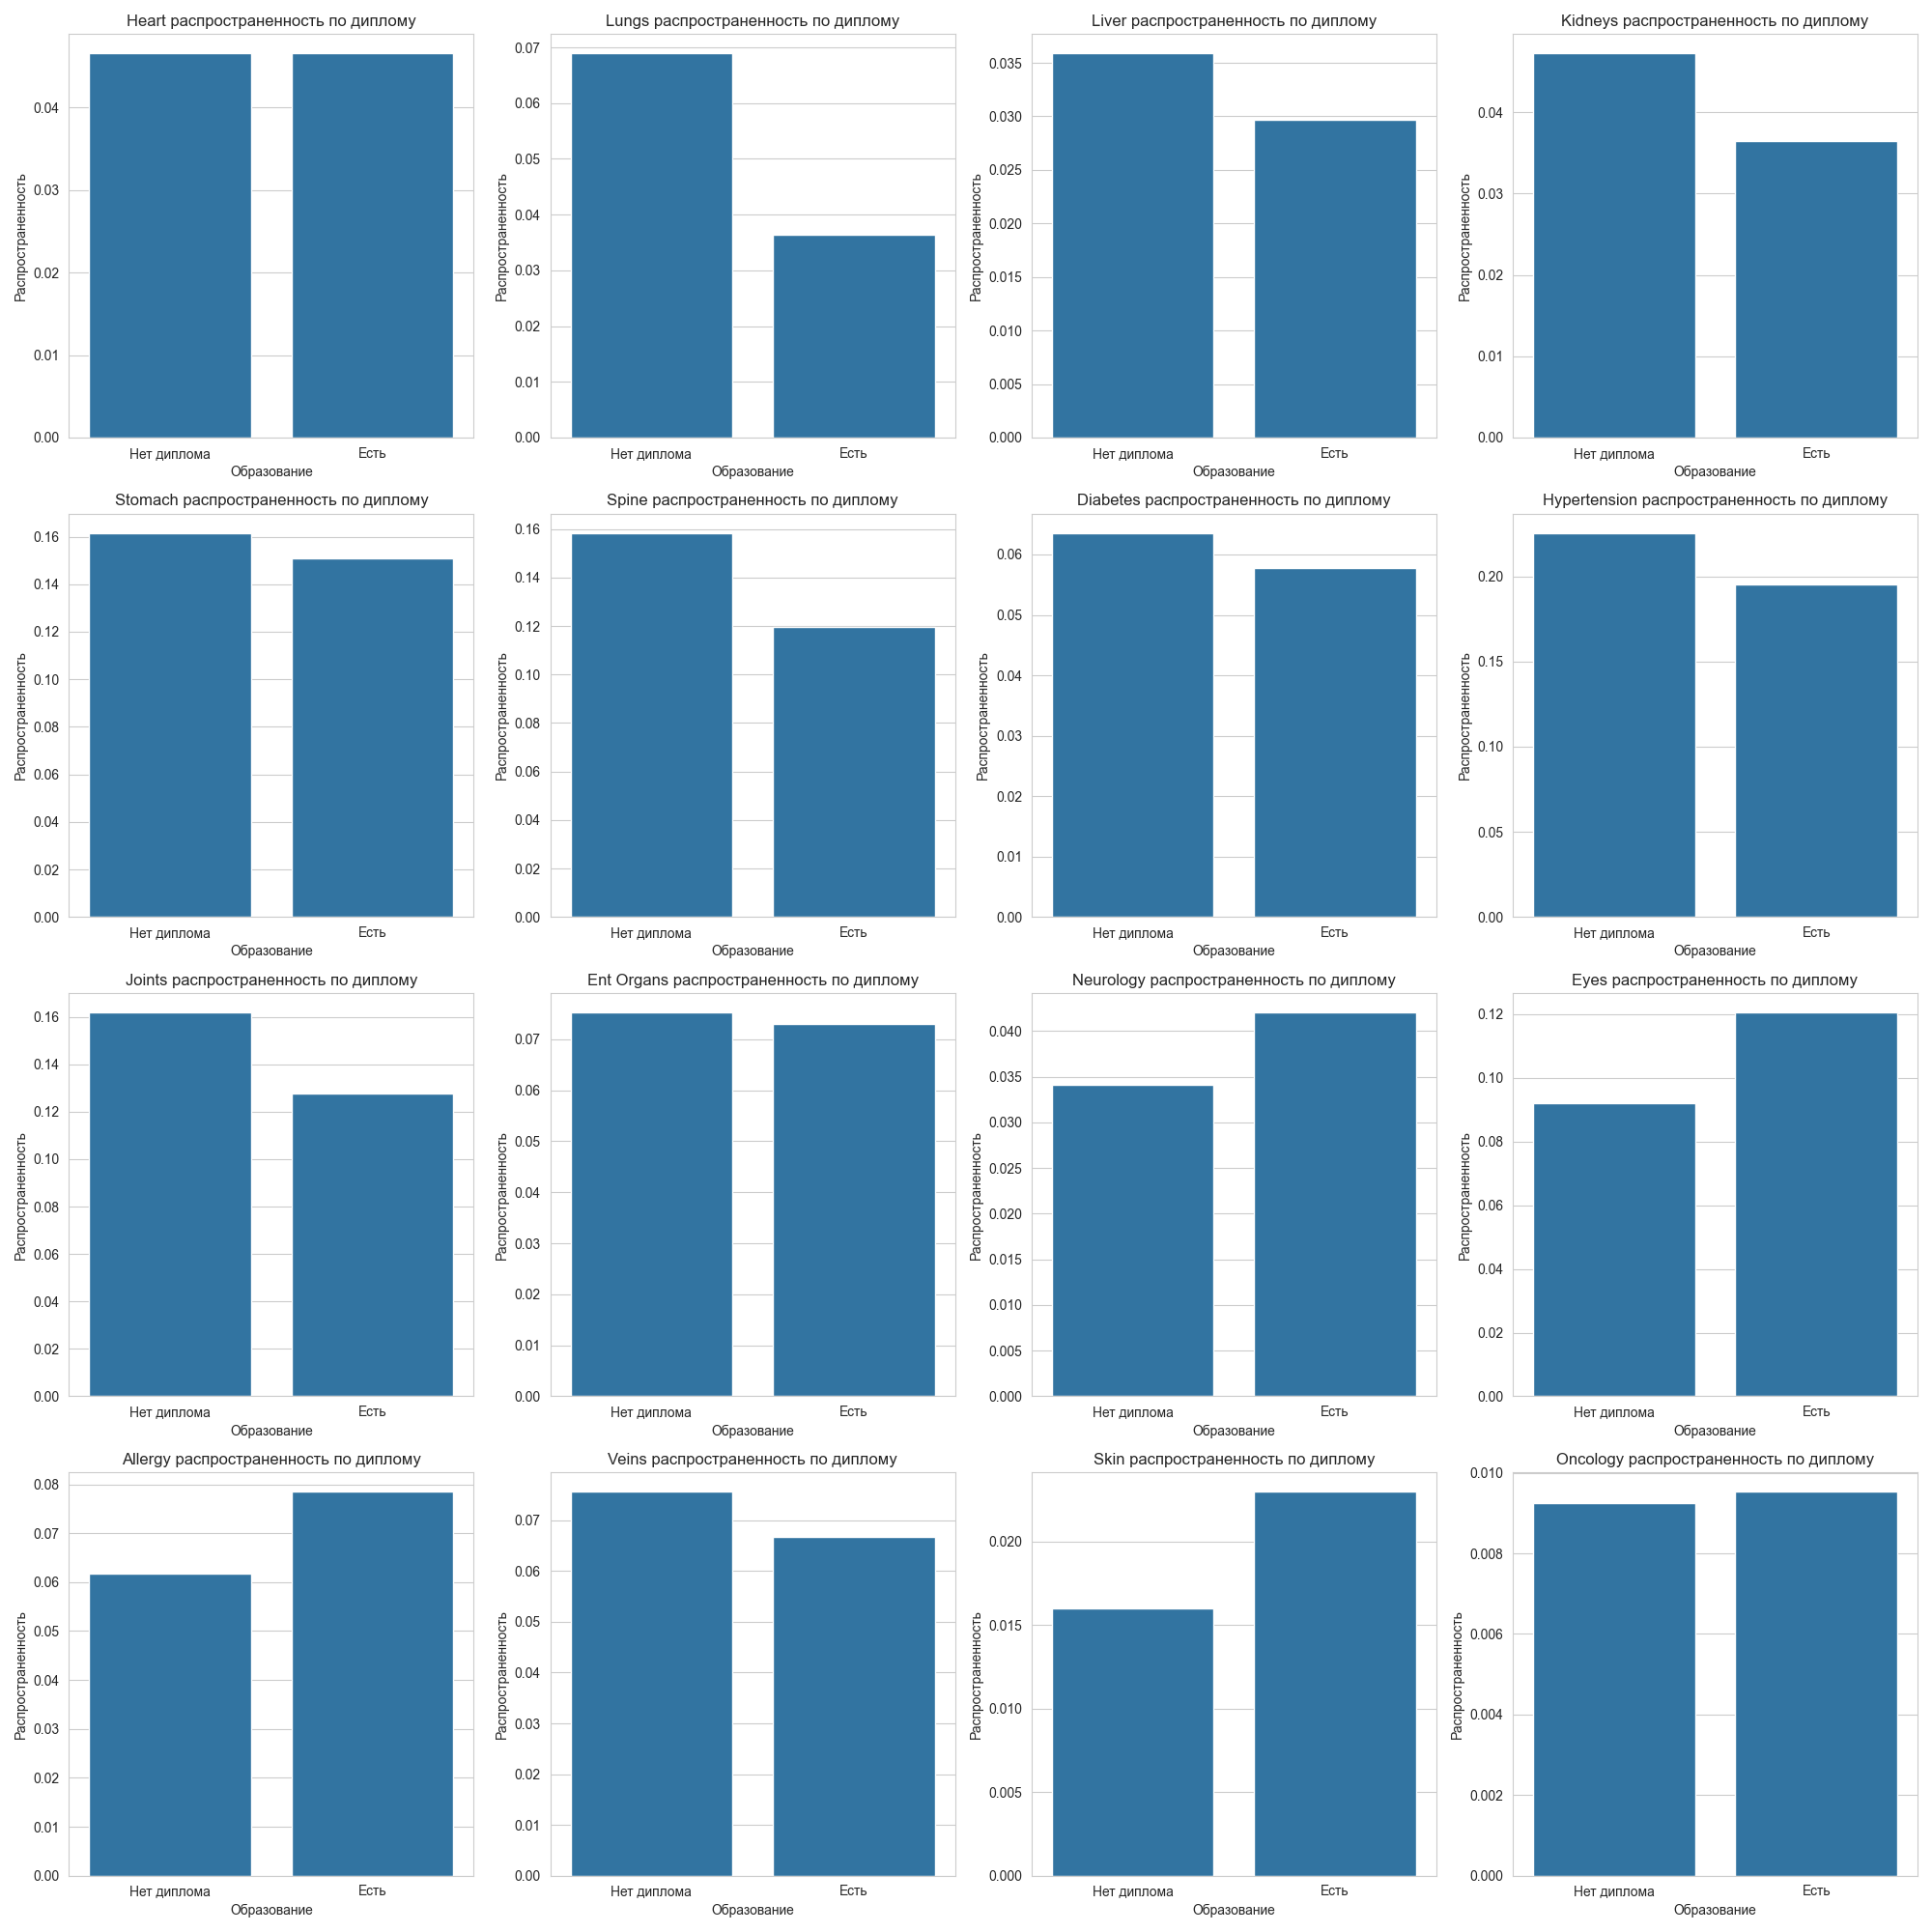
\includegraphics[width=0.8\textwidth]{assets/disease_spread_by_diploma.png}
\end{center}

\begin{center}
    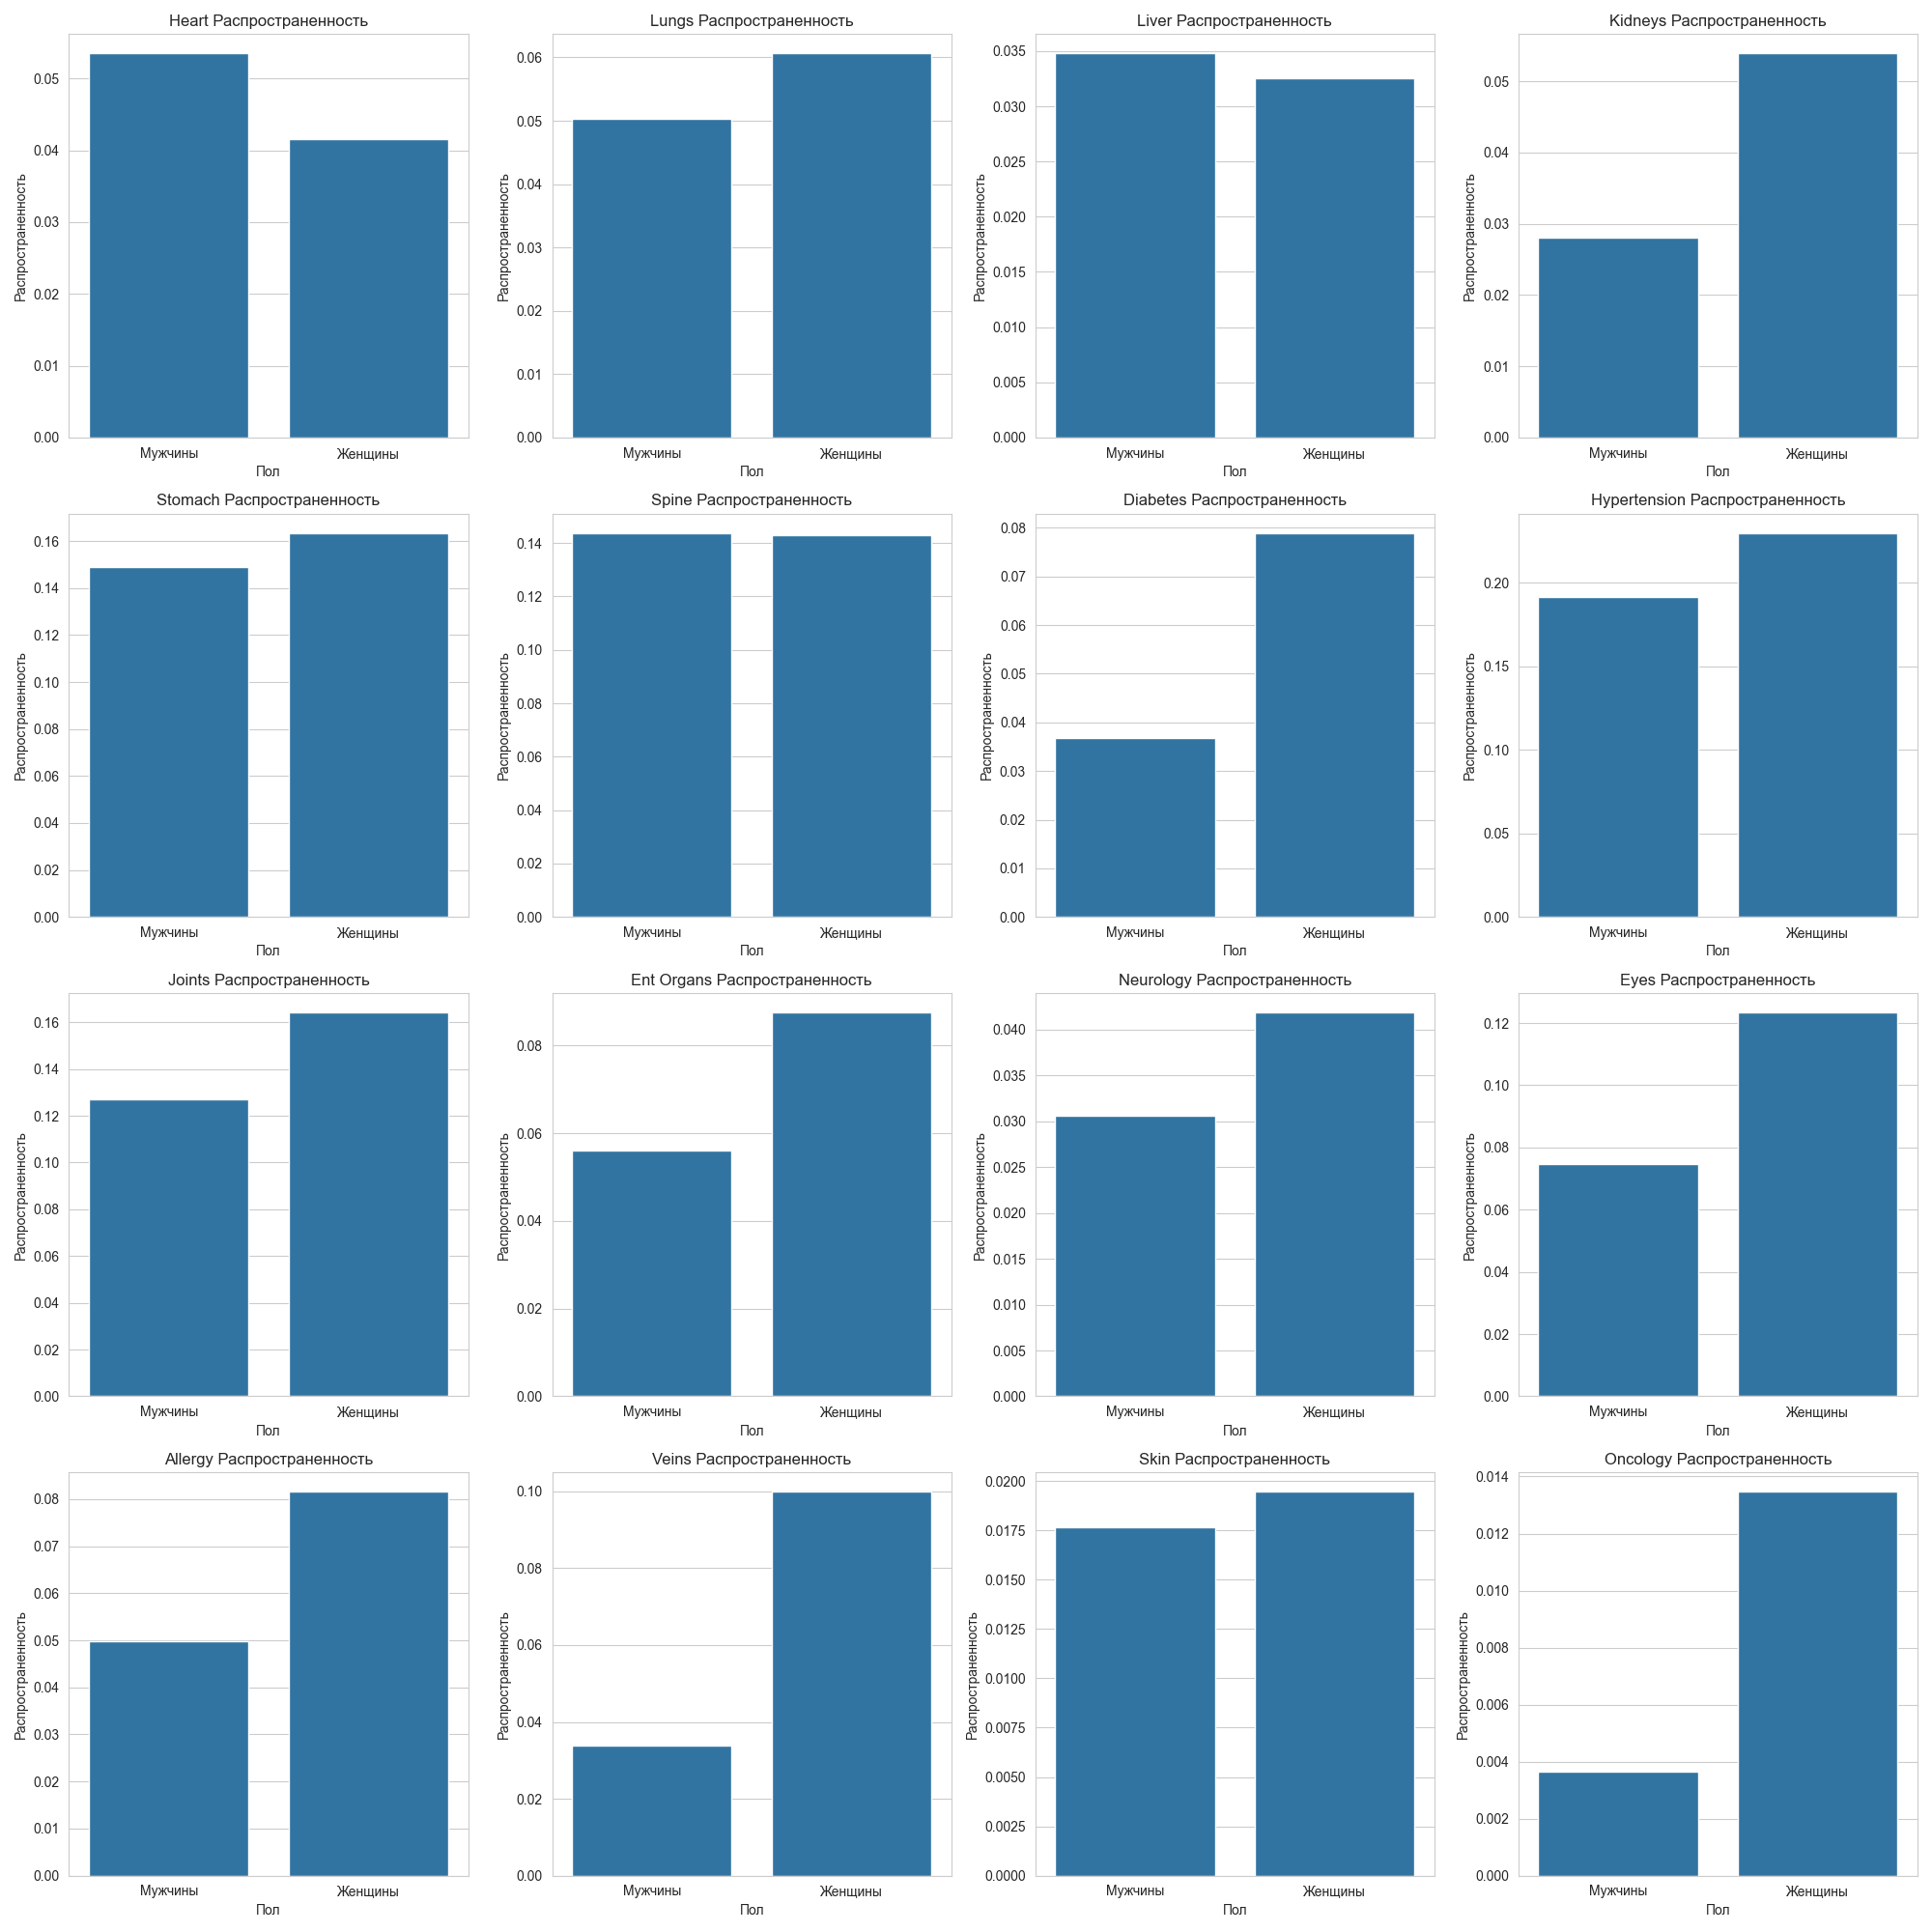
\includegraphics[width=0.8\textwidth]{assets/disease_spread_by_sex.png}
\end{center}

\newpage{}

\section{Обзор методов}

\newpage{}

\section{Пробит модель}

\newpage{}

\section{Мэтчинг}

\newpage{}

\section{Double ML}

\begin{center}
    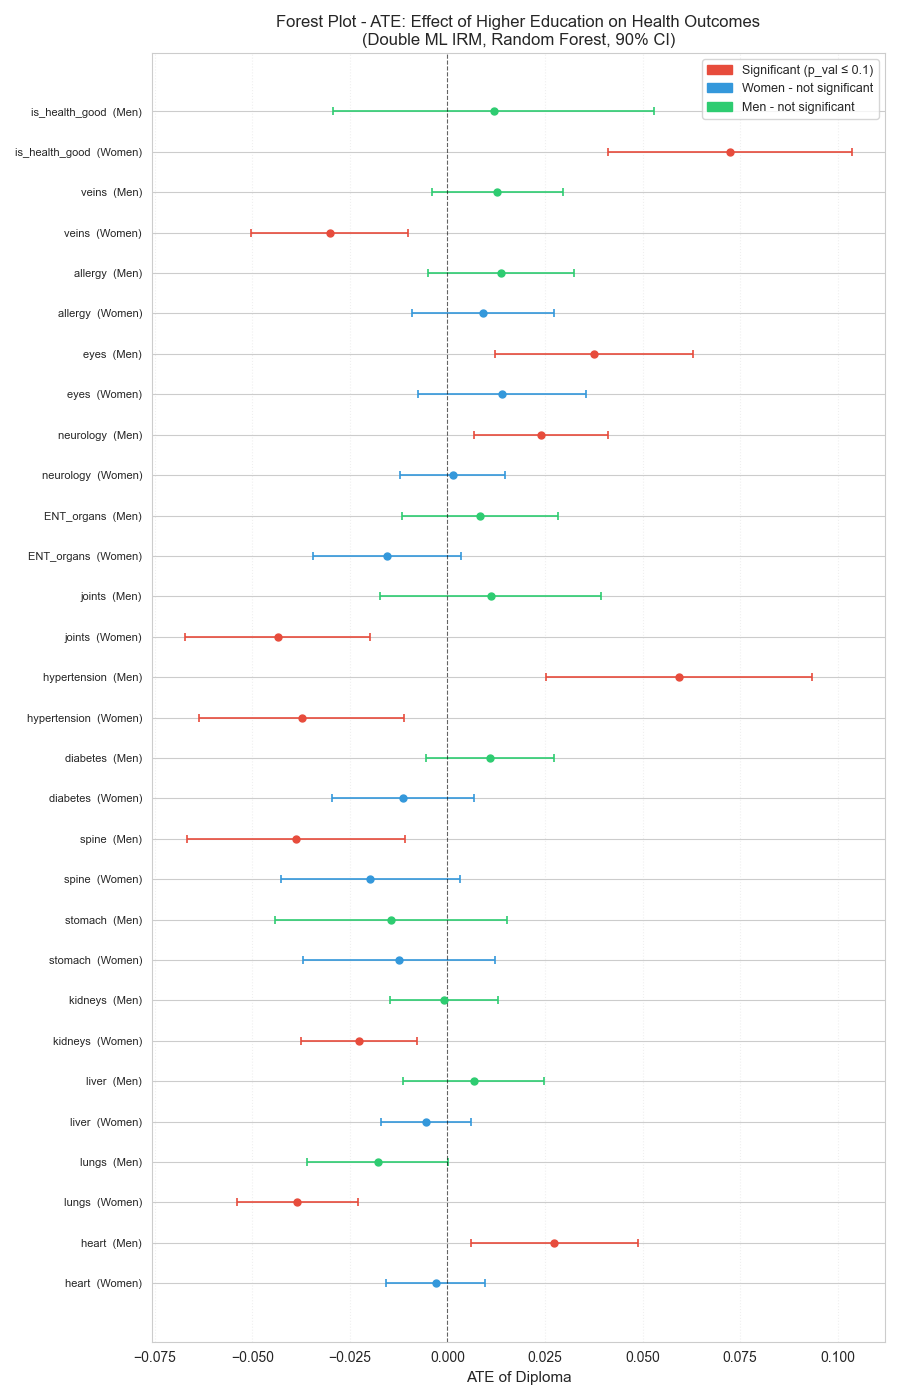
\includegraphics[width=0.8\textwidth]{assets/dml_forest_plot_ate.png}
\end{center}

\begin{center}
    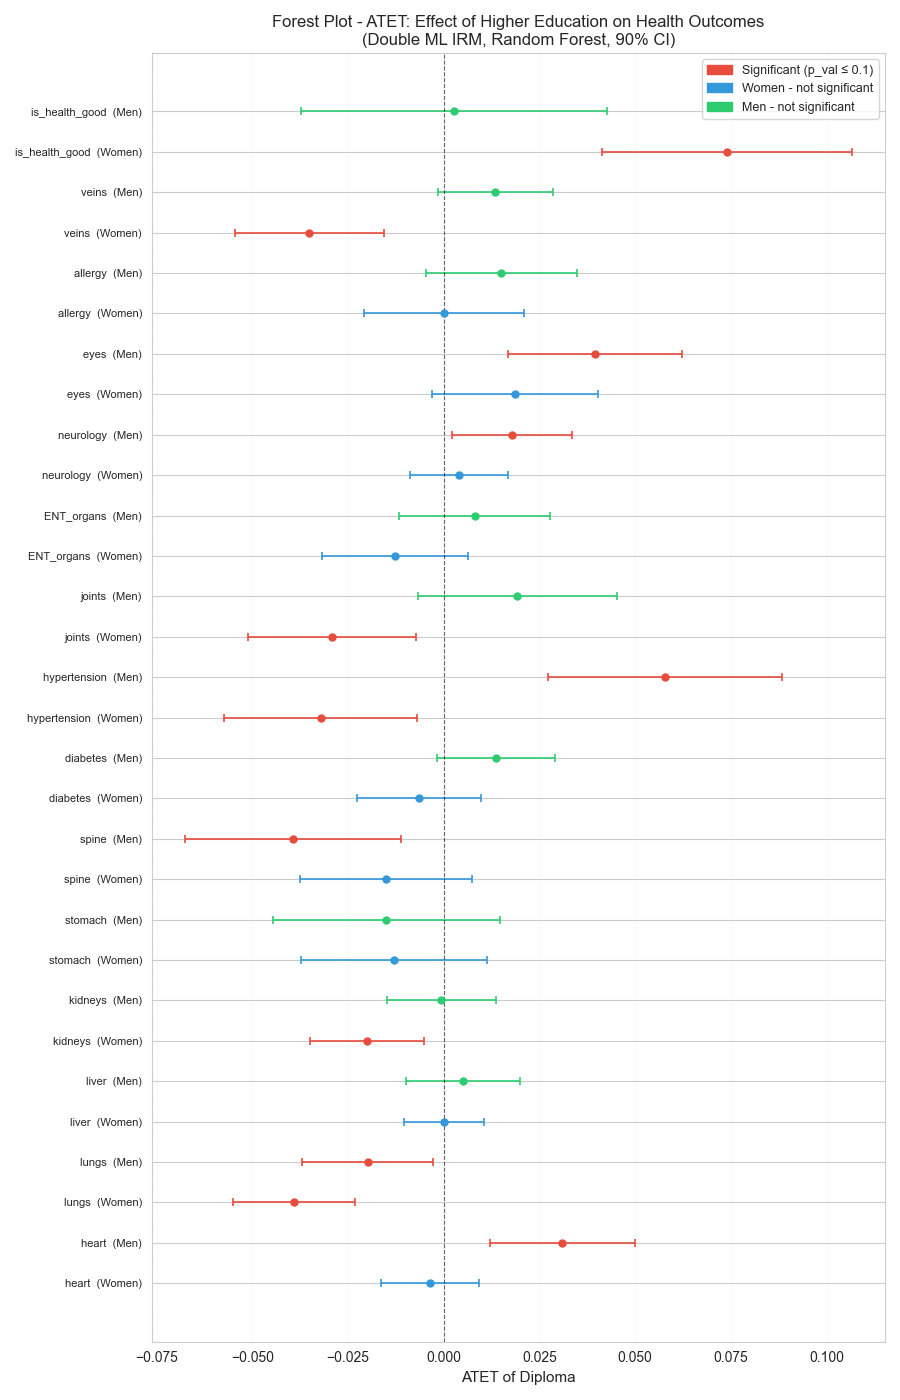
\includegraphics[width=0.8\textwidth]{assets/dml_forest_plot_atet.png}
\end{center}

\begin{center}
    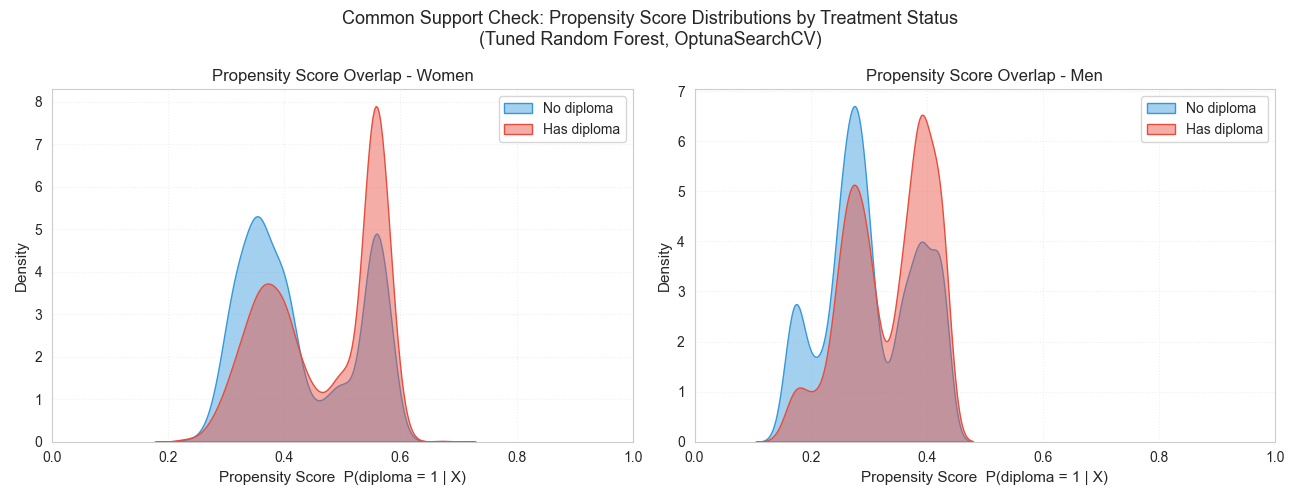
\includegraphics[width=0.8\textwidth]{assets/dml_propensity_score.png}
\end{center}

\begin{center}
    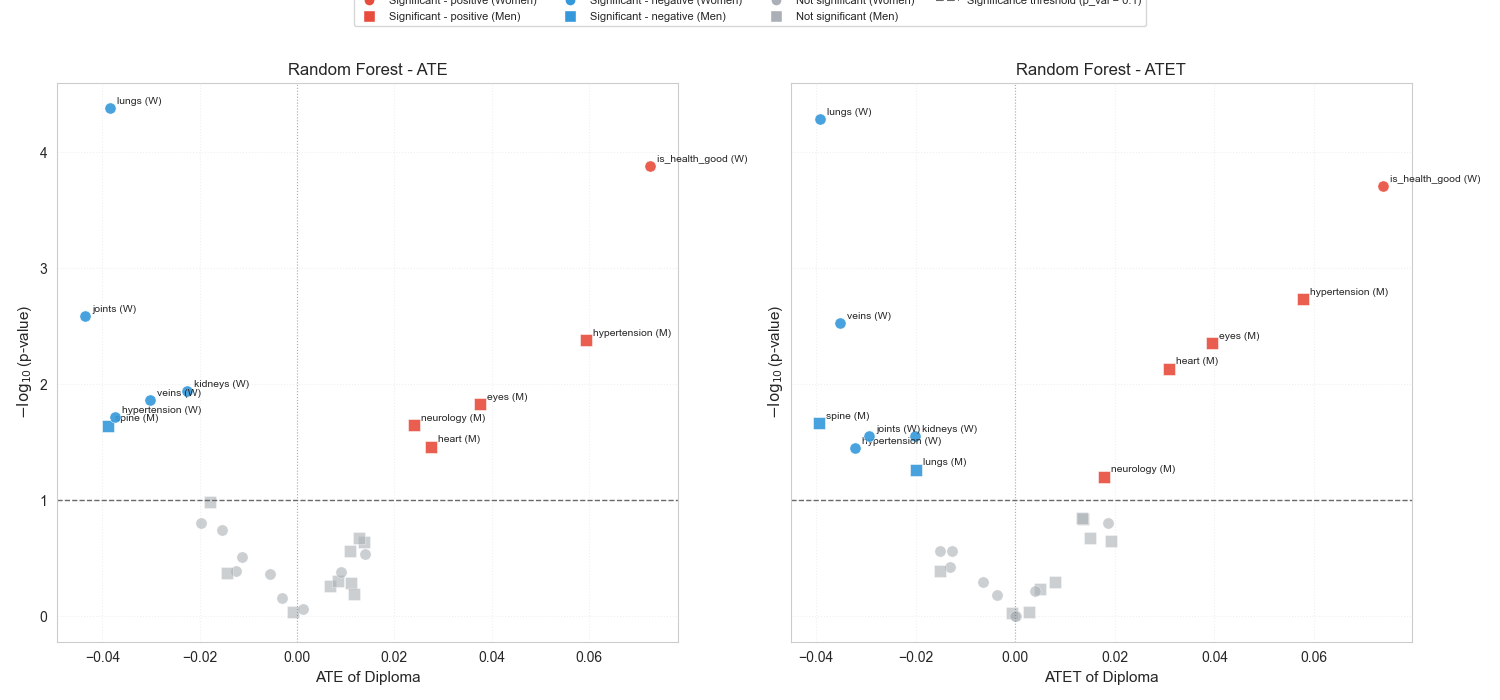
\includegraphics[width=0.8\textwidth]{assets/dml_volcano_plot.png}
\end{center}

\newpage{}

\section{Выводы}

\newpage{}

\tableofcontents{}

\end{document}
